\subsection{Modifica dataset visualizzato}

\begin{figure}[H]
    \centering
    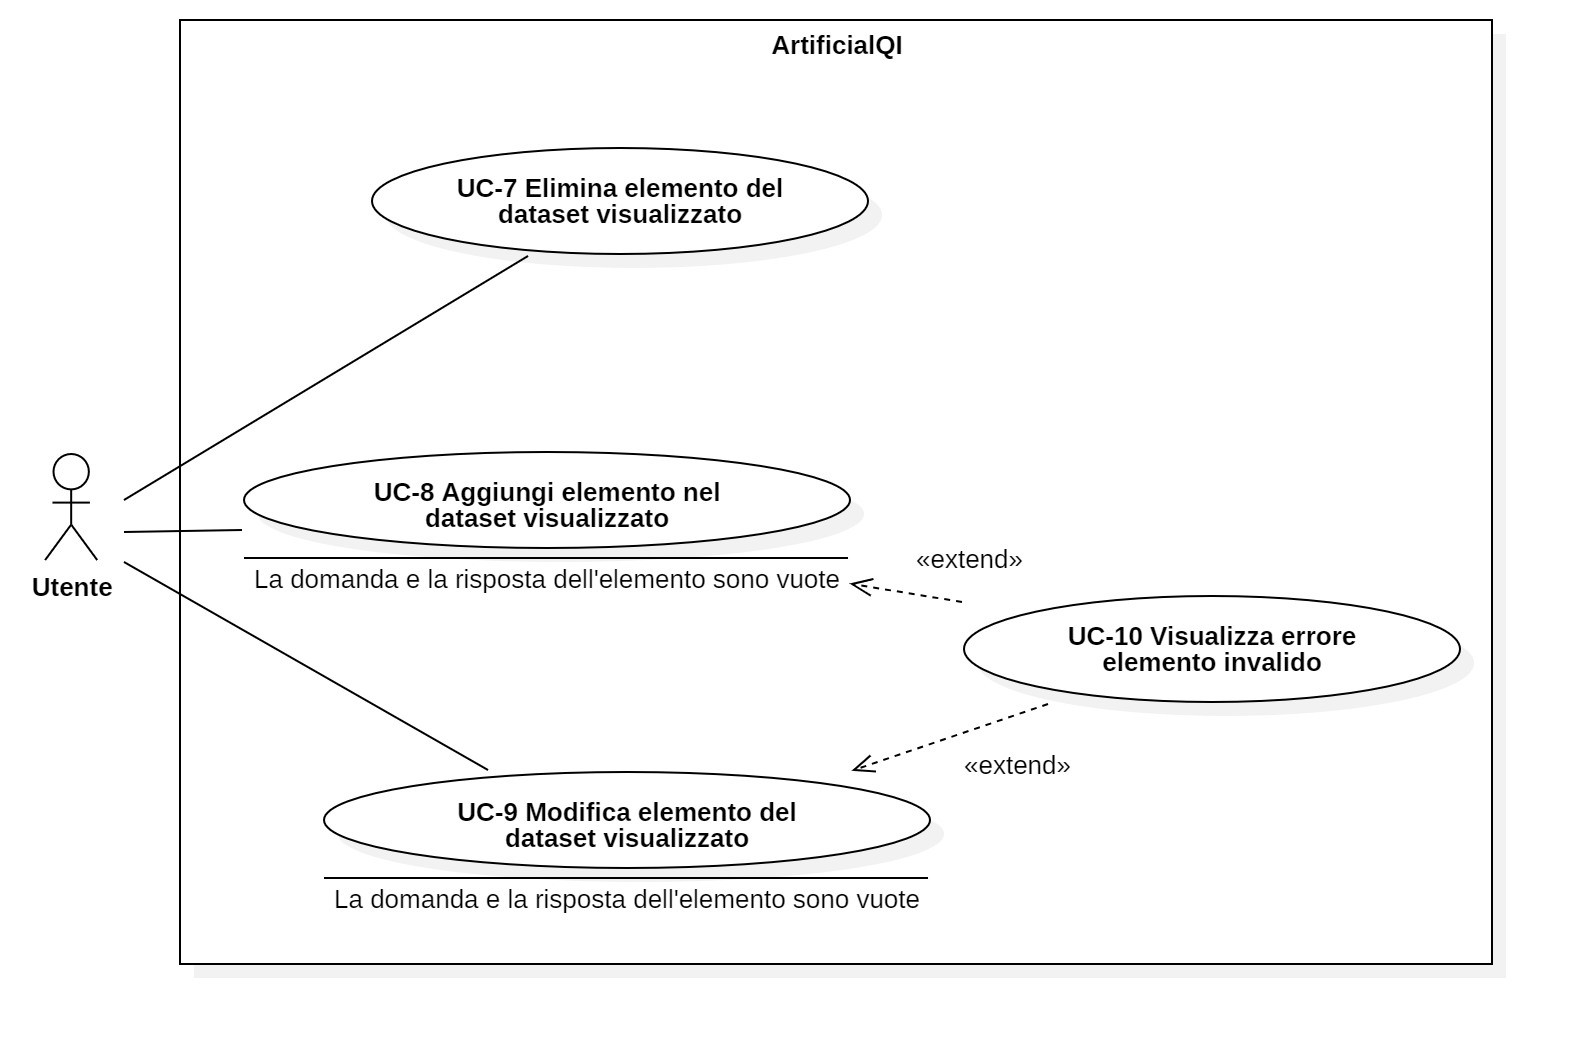
\includegraphics[scale=0.5]{Sezioni/UseCase/Immagini/ModificaDatasetVisualizzato.png}
    \caption{Diagramma modifica dataset visualizzato.}
\end{figure}



\begin{usecase}{UC-5}{Elimina elemento del dataset visualizzato}
    \label{uc:UC-5}
    
    \req{\hyperref[ru:RUO-1]{RUO-1}} 

    \pre{
        \item L'utente sta visualizzando la pagina del dataset caricato che contiene l'elemento da eliminare 
    }

    \post{
        \item L'elemento viene eliminato dal dataset visualizzato
    }
    
    \actor{Utente}

    \subactors{}

    \trigger{L'utente vuole eliminare un elemento contenuto nel dataset visualizzato}

    \inc{}

    \base{}

    \scenario{

        \item L'utente richiede l'eliminazione dell'elemento
        \item Il sistema richiede la conferma dell'eliminazione
        \item L'utente conferma l'eliminazione
        \item Il sistema elimina l'elemento dal dataset caricato
    }

    \subscenario{
        \item[3.1] L'utente annulla l'eliminazione:
        \begin{itemize}
            \item Il sistema annulla l'operazione
            \item Il sistema avvisa l'utente del corretto annullamento
        \end{itemize}
    }

\end{usecase}


\begin{usecase}{UC-6}{Aggiungi elemento nel dataset visualizzato}
    \label{uc:UC-6}
    
    \req{\hyperref[ru:RUO-1]{RUO-1}}

    \pre{
        \item L'utente sta visualizzando una pagina del dataset caricato \hyperref[uc:UC-1]{UC-1}
    }

    \post{
        \item L'elemento viene inserito nel dataset visualizzato
    }
    
    \actor{Utente}

    \subactors{}
    
    \trigger{L'utente vuole inserire un nuovo elemento nel dataset visualizzato}
    
    \inc{}

    \base{}

    \scenario{
        \item L'utente richiede l'inserimento di un nuovo elemento nel dataset visualizzato
        \item L'utente specifica la domanda e/o la risposta per il nuovo elemento
        \item L'utente conferma l'inserimento del nuovo elemento
        \item Il sistema verifica la correttezza dell'elemento
        \item Il sistema aggiunge l'elemento al dataset visualizzato
    }

    \subscenario{
        \item[3.1] L'utente annulla l'inserimento:
        \begin{itemize}
            \item Il sistema annulla l'operazione
        \end{itemize}
        \item[4.1] La domanda e la risposta sono vuote:
        \begin{itemize}
            \item \hyperref[uc:UC-8]{UC-8}
        \end{itemize}
    }

\end{usecase}

\begin{usecase}{UC-7}{Modifica elemento del dataset visualizzato}
    \label{uc:UC-7}
    
    \req{\hyperref[ru:RUO-1]{RUO-1}} 

    \pre{
        \item L'utente sta visualizzando la pagina del dataset caricato che contiene l'elemento da modificare 
    }

    \post{
        \item La modifica dell'elemento viene registrata nel dataset visualizzato
    }
    
    \actor{Utente}

    \subactors{}
    
    \trigger{L'utente vuole modificare un elemento del dataset visualizzato}
    
    \inc{}

    \base{}

    \scenario{
        \item L'utente richiede la modifica di un elemento
        \item L'utente modifica la domanda e/o la risposta dell'elemento
        \item L'utente conferma la modifica
        \item Il sistema verifica la correttezza della modifica
        \item Il sistema registra la modifica nel dataset visualizzato
    }

    \subscenario{
        \item[3.1] L'utente annulla l'inserimento:
        \begin{itemize}
            \item Il sistema annulla l'operazione
        \end{itemize}
        \item[4.1] La domanda e la risposta sono vuote:
        \begin{itemize}
            \item \hyperref[uc:UC-8]{UC-8}
        \end{itemize}
    }

\end{usecase}

\begin{usecase}{UC-8}{Visualizza errore elemento invalido}
    \label{uc:UC-8}
    
    \req{}

    \pre{
        \item Il sistema ha verificato la presenza di un elemento invalido
    }

    \post{
        \item L'utente viene avvisato e viene guidato nella corretta compilazione dell'elemento
    }
    
    \actor{Utente}

    \subactors{}

    \trigger{Domanda e riposta di un elemento sono entrambe vuote}
    
    \inc{}

    \base{}

    \scenario{
        \item Viene visualizzato un messaggio che spiega la presenza di un elemento invalido 
        \item Viene indicato come compilare correttamente un elemento
    }

    \subscenario{}

\end{usecase}


